\chapter{The Birch and Swinnerton-Dyer Conjecture}
\label{ch:birch}

\medskip\noindent\textbf{Prerequisites.} This chapter assumes a solid grounding in abstract algebra---including groups, rings, and fields---as well as some basic number theory and familiarity with complex analysis. Readers who need a refresher on modular arithmetic or the structure of finite fields should consult the Mathematical Preliminaries appendix. The group law on elliptic curves is developed from scratch, so no prior knowledge of algebraic geometry is required.

\noindent\textbf{Key Ideas.}
\begin{itemize}
  \item An \emph{elliptic curve} $E: y^2 = x^3 + ax + b$ has a group structure on its rational points $E(\mathbb{Q})$.
  \item The \emph{rank} of $E(\mathbb{Q})$ measures how many independent rational points exist---it is the deepest arithmetic invariant.
  \item The BSD conjecture predicts the rank from the \emph{$L$-function} $L(E,s)$: $\operatorname{ord}_{s=1} L(E,s) = \operatorname{rank}(E(\mathbb{Q}))$.
  \item Known for analytic rank $\le 1$ (Gross--Zagier, Kolyvagin), but open in general.
\end{itemize}

\bigskip

\section{Introduction}
\label{sec:bsd-intro}

The Birch and Swinnerton-Dyer conjecture (BSD) stands as one of the deepest and most consequential open problems in mathematics. At its heart lies a deceptively simple question: \emph{How many rational solutions does an elliptic curve have?} The conjecture asserts that the answer to this arithmetic question is encoded in an analytic object---an $L$-function---that one constructs from the curve's behavior modulo primes. The bridge between arithmetic and analysis that BSD proposes is so profound that it touches nearly every branch of modern number theory, from the Langlands program to the theory of modular forms, from arithmetic geometry to computational number theory.

The story of BSD begins not with a theoretical insight, but with a computer. In the early 1960s, Bryan Birch and Peter Swinnerton-Dyer used the EDSAC machine at the University of Cambridge to compute the number of points on elliptic curves over finite fields. They plotted their data on logarithmic scales and observed a striking pattern: the slope of the resulting line appeared to equal the rank of the elliptic curve. This empirical observation, born from one of the earliest applications of electronic computers to pure mathematics, crystallized into a conjecture that has guided research for over half a century.

The importance of BSD can hardly be overstated. It is one of only two Millennium Prize Problems (along with the Riemann hypothesis) whose resolution would immediately imply deep structural results in number theory. The full BSD conjecture implies the weak BSD conjecture, which in turn implies finiteness of the Tate--Shafarevich group---a statement that would revolutionize our understanding of rational points on algebraic varieties. Moreover, the tools developed in pursuit of BSD---Euler systems, Heegner points, the modularity theorem---have themselves transformed mathematics.

The Birch and Swinnerton-Dyer conjecture remains open in full generality. The most we can prove are results for curves of analytic rank 0 and 1, thanks to the monumental work of Coates and Wiles, Gross and Zagier, and Kolyvagin. But the full conjecture, relating the order of vanishing of $L(E,s)$ at $s=1$ to the algebraic rank of $E(\mathbb{Q})$, and giving an exact formula for the leading coefficient, remains one of the great challenges of twenty-first-century mathematics.

In this chapter, we develop the theory of elliptic curves, define their $L$-functions, state the BSD conjecture precisely, and survey the evidence and partial results. We begin with the geometric foundations: elliptic curves as algebraic curves, their group law, and the Mordell--Weil theorem. We then turn to the analytic side: reduction modulo primes, Hasse's theorem, and the $L$-function. The climax is the statement of BSD itself and the remarkable theorems that support it.

\section{Elliptic Curves: Definitions and Examples}
\label{sec:elliptic-curves}

\subsection{Weierstrass Equations}

An elliptic curve is a smooth projective algebraic curve of genus 1 with a specified rational point. Over a field $K$ of characteristic different from 2 or 3, every such curve can be written in \emph{short Weierstrass form}.

\begin{definition}
An \textit{elliptic curve} over a field $K$ is a smooth, projective, genus-1 curve $E$ over $K$ together with a distinguished $K$-rational point $\mathcal{O} \in E(K)$. In short Weierstrass form, $E$ is given by the affine equation
\[
E:\; y^2 = x^3 + ax + b, \qquad a, b \in K,
\]
together with the point at infinity $\mathcal{O}$. The \textit{discriminant} of the curve is
\[
\Delta = -16(4a^3 + 27b^2).
\]
\end{definition}

The condition $\Delta \neq 0$ is equivalent to the curve being smooth, meaning the polynomial $x^3 + ax + b$ has no repeated roots. When $\Delta = 0$, the curve has a singularity (a node or a cusp) and is not an elliptic curve in the strict sense.

\begin{definition}
The \textit{$j$-invariant} of an elliptic curve $E: y^2 = x^3 + ax + b$ is
\[
j(E) = -1728 \cdot \frac{(4a)^3}{\Delta} = \frac{-6912\, a^3}{\Delta}.
\]
Two elliptic curves over an algebraically closed field are isomorphic if and only if they have the same $j$-invariant.
\end{definition}

The $j$-invariant classifies elliptic curves up to isomorphism over algebraically closed fields. Over a general field $K$, curves with the same $j$-invariant may not be isomorphic over $K$; they belong to the same \emph{isogeny class}.

\subsection{The General Weierstrass Equation}

In full generality, without assumptions on the characteristic, an elliptic curve is given by the \emph{general Weierstrass equation}:
\[
y^2 + a_1 xy + a_3 y = x^3 + a_2 x^2 + a_4 x + a_6,
\]
where $a_1, a_2, a_3, a_4, a_6 \in K$. The change of variables
\[
x = u^2 x' + r, \qquad y = u^3 y' + u^2 s x' + t
\]
(with $u \in K^\times$ and $r, s, t \in K$) transforms one Weierstrass equation into another. By choosing appropriate substitutions, the equation can be brought to short Weierstrass form when $\operatorname{char}(K) \notin \{2, 3\}$.

The \emph{discriminant} $\Delta$ and $j$-invariant are defined using the standard invariants:
\begin{align}
b_2 &= a_1^2 + 4a_2, \\
b_4 &= a_1 a_3 + 2a_4, \\
b_6 &= a_3^2 + 4a_6, \\
b_8 &= a_1^2 a_6 - a_1 a_3 a_4 + a_2 a_6 + a_2 a_3^2/4 - a_4^2.
\end{align}
Then $\Delta = -b_2^2 b_8 - 8b_4^3 - 27b_6^2 + 9b_2 b_4 b_6$ and $c_4 = b_2^2 - 24b_4$, with $j = c_4^3/\Delta$.

\subsection{Smoothness and the Point at Infinity}

The point at infinity $\mathcal{O}$ is the unique point on the projective closure of $E$ that lies on the line at infinity. In projective coordinates $[X : Y : Z]$, the Weierstrass equation becomes:
\[
Y^2 Z + a_1 XYZ + a_3 YZ^2 = X^3 + a_2 X^2 Z + a_4 XZ^2 + a_6 Z^3.
\]
Setting $Z = 0$, we find $X^3 = 0$, so $X = 0$. The point at infinity is $\mathcal{O} = [0 : 1 : 0]$. This point plays a fundamental role as the identity element of the group law.

The smoothness condition $\Delta \neq 0$ ensures that every point on the curve has a well-defined tangent line. This is essential for the chord-tangent construction of the group law.

\begin{example}
Consider $E: y^2 = x^3 - x = x(x-1)(x+1)$ over $\mathbb{Q}$. We have $a = -1$, $b = 0$, and
\[
\Delta = -16(4(-1)^3 + 0) = 64 \neq 0.
\]
The curve is smooth. The $j$-invariant is $j(E) = -1728 \cdot (-4)^3/64 = -1728 \cdot (-64)/64 = 1728$. The rational points visible in $\mathbb{R}$ are $(0,0)$, $(1,0)$, $(-1,0)$, and $\mathcal{O}$.
\end{example}

\begin{example}
The curve $E: y^2 = x^3 + 1$ has $a = 0$, $b = 1$, $\Delta = -432$, and $j(E) = 0$. This curve has the remarkable property that it is isomorphic to its own Galois conjugate over $\mathbb{Q}(\sqrt{-3})$, and it has complex multiplication by $\mathbb{Z}[\omega]$ where $\omega = e^{2\pi i/3}$.
\end{example}

\begin{example}
Consider $E: y^2 = x^3 - 25x$. Here $a = -25$, $b = 0$, $\Delta = -16 \cdot 4 \cdot (-25)^3 = 1{,}000{,}000$, and $j(E) = 1728$. The rational points include $(0,0)$, $(5,0)$, $(-5,0)$, and $\mathcal{O}$.
\end{example}

\subsection{Real Points and Visualization}

When $E$ is defined over $\mathbb{R}$, we can plot its real points. The topology of $E(\mathbb{R})$ depends on whether $x^3 + ax + b$ has one or three real roots:
\begin{itemize}
\item If $\Delta > 0$ (three real roots), then $E(\mathbb{R})$ has two connected components: one compact oval and one unbounded branch.
\item If $\Delta < 0$ (one real root), then $E(\mathbb{R})$ consists of a single connected component (unbounded).
\end{itemize}

In both cases, $E(\mathbb{R})$ is a Lie group diffeomorphic to either $S^1$ or $S^1 \times \mathbb{Z}/2\mathbb{Z}$. The compact oval, when present, resembles a circle, and the group law on it is essentially addition of angles.

\subsection{Examples over Finite Fields}

For each prime $p$ where $p \nmid \Delta$, we reduce the equation of $E$ modulo $p$ to obtain a curve $\widetilde{E}$ over $\mathbb{F}_p$. The set $\widetilde{E}(\mathbb{F}_p)$ of $\mathbb{F}_p$-rational points is always finite, and its size is closely related to the $L$-function of $E$. Computing $|\widetilde{E}(\mathbb{F}_p)|$ is a central task in computational number theory and lies at the heart of the BSD conjecture.

\begin{example}
Let $E: y^2 = x^3 - x$ and $p = 5$. Reducing modulo 5, we count solutions:
\begin{center}
\begin{tabular}{c|c}
$x \bmod 5$ & $x^3 - x \bmod 5$ \\ \hline
0 & 0 \\
1 & 0 \\
2 & $8 - 2 = 6 \equiv 1$ \\
3 & $27 - 3 = 24 \equiv 4$ \\
4 & $64 - 4 = 60 \equiv 0$
\end{tabular}
\end{center}
For $x = 2$: $y^2 \equiv 1$ gives $y \equiv 1, 4$ (2 points). For $x = 3$: $y^2 \equiv 4$ gives $y \equiv 2, 3$ (2 points). For $x = 0, 1, 4$: $y^2 \equiv 0$ gives $y \equiv 0$ (1 point each). Including $\mathcal{O}$:
\[
\#\widetilde{E}(\mathbb{F}_5) = 3 \cdot 1 + 2 \cdot 2 + 1 = 8.
\]
Hasse's bound gives $|8 - 6| \le 2\sqrt{5} \approx 4.47$. $\checkmark$
\end{example}

\section{The Group Law}
\label{sec:group-law}

One of the most remarkable features of elliptic curves is that their rational points carry a natural group structure. This group law has a beautiful geometric description and makes the study of $E(K)$ a problem in group theory.

\subsection{The Chord-Tangent Construction}

Let $E$ be an elliptic curve over a field $K$, and let $P, Q \in E(K)$ be two rational points (possibly equal). The group law is defined as follows:

\begin{enumerate}
\item \textbf{Line through $P$ and $Q$:} Draw the line $\ell$ through $P$ and $Q$ (if $P = Q$, take the tangent line to $E$ at $P$).
\item \textbf{Third intersection:} By Bézout's theorem, $\ell$ meets $E$ in exactly three points (counted with multiplicity), say $P$, $Q$, and $R$.
\item \textbf{Reflection:} Define $P \oplus Q$ to be the reflection of $R$ across the $x$-axis. That is, if $R = (x_0, y_0)$, then $P \oplus Q = (x_0, -y_0)$.
\end{enumerate}

The point at infinity $\mathcal{O}$ is the identity element: $P \oplus \mathcal{O} = P$ for all $P$. The inverse of $P = (x, y)$ is $-P = (x, -y)$.

\begin{checkyou}
\begin{enumerate}
\item Why is the point at infinity $\mathcal{O} = [0:1:0]$ the identity element of the group law? What happens geometrically when you draw a line through a point $P$ and $\mathcal{O}$?
\item Why must the third intersection point be reflected across the $x$-axis to obtain the group sum?
\end{enumerate}
\end{checkyou}

\begin{figure}[htbp]
\centering
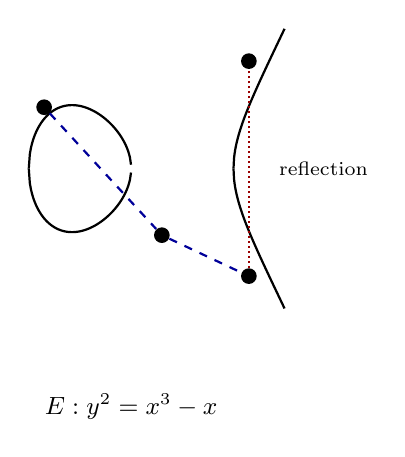
\begin{tikzpicture}[
  scale=1.3,
  dot/.style={circle, fill, inner sep=2pt},
  label/.style={font=\small},
  arr/.style={->, thick, gray}
]
  \draw[thick, domain=-1:0, samples=100] plot (\x, {sqrt(\x*\x*\x - \x)});
  \draw[thick, domain=-1:0, samples=100] plot (\x, {-sqrt(\x*\x*\x - \x)});
  \draw[thick, domain=1:1.5, samples=100] plot (\x, {sqrt(\x*\x*\x - \x)});
  \draw[thick, domain=1:1.5, samples=100] plot (\x, {-sqrt(\x*\x*\x - \x)});

  \node[dot, label={[label]above left:$P$}] (P) at (-0.85, 0.6) {};
  \node[dot, label={[label]above right:$Q$}] (Q) at (0.3, -0.65) {};
  \node[dot, label={[label]below:$R$}] (R) at (1.15, -1.05) {};
  \node[dot, label={[label]above:$P \oplus Q$}] (PQ) at (1.15, 1.05) {};

  \draw[thick, dashed, blue!60!black] (P) -- (Q) -- (R) -- cycle;
  \draw[thick, densely dotted, red!60!black] (R) -- (PQ);

  \node[font=\scriptsize, anchor=west] at (1.35, 0) {reflection};
  \node[font=\small, anchor=north] at (0,-2.1) {$E: y^2 = x^3 - x$};
\end{tikzpicture}
\caption{The chord-tangent group law on $E: y^2 = x^3 - x$. The line through $P$ and $Q$ meets $E$ at a third point $R$; reflecting $R$ across the $x$-axis gives $P \oplus Q$.}
\label{fig:chord-tangent}
\end{figure}

\begin{proposition}[Associativity]
The operation $\oplus$ defines an abelian group on $E(K)$. In particular, it is associative: $(P \oplus Q) \oplus R = P \oplus (Q \oplus R)$.
\end{proposition}

The proof of associativity is notoriously difficult to carry out by direct algebraic computation. A cleaner proof uses the theory of divisors, which we sketch below.

\subsection{Algebraic Formulas for Addition}

Let $E: y^2 = x^3 + ax + b$ and let $P = (x_1, y_1)$, $Q = (x_2, y_2)$ with $P, Q, \mathcal{O}$ not all equal.

\textbf{Case 1: $P \neq \pm Q$ (generic addition).}
The slope of the line through $P$ and $Q$ is
\[
\lambda = \frac{y_2 - y_1}{x_2 - x_1}.
\]
Then $P \oplus Q = (x_3, y_3)$ where
\begin{align}
x_3 &= \lambda^2 - x_1 - x_2, \label{eq:x3-add} \\
y_3 &= \lambda(x_1 - x_3) - y_1. \label{eq:y3-add}
\end{align}

\textbf{Case 2: $Q = -P$ (i.e., $x_1 = x_2$, $y_1 = -y_2$).}
The line is vertical, meeting $E$ only at $P$, $-P$, and $\mathcal{O}$. Thus $P \oplus Q = \mathcal{O}$.

\textbf{Case 3: $P = Q$ (doubling).}
Taking the tangent line at $P = (x_1, y_1)$ (with $y_1 \neq 0$), the slope is
\[
\lambda = \frac{3x_1^2 + a}{2y_1}.
\]
Then $2P = (x_3, y_3)$ with
\begin{align}
x_3 &= \lambda^2 - 2x_1, \label{eq:x3-double} \\
y_3 &= \lambda(x_1 - x_3) - y_1. \label{eq:y3-double}
\end{align}

If $P = (x_1, 0)$ (a point of order 2), then $2P = \mathcal{O}$.

\begin{example}
Let $E: y^2 = x^3 - x$ and $P = (0, 0)$. Since $P$ has $y = 0$, it is a 2-torsion point: $2P = \mathcal{O}$.

Now let $Q = (2, \sqrt{6})$. (This point is not rational, but we can still compute over $\mathbb{R}$.) The slope of the line through $P = (0,0)$ and $Q = (2, \sqrt{6})$ is $\lambda = \sqrt{6}/2$. Then
\[
x_3 = \frac{6}{4} - 0 - 2 = -\frac{1}{2}, \qquad y_3 = \frac{\sqrt{6}}{2}\left(0 + \frac{1}{2}\right) - 0 = \frac{\sqrt{6}}{4}.
\]
So $P \oplus Q = (-1/2, \sqrt{6}/4)$.
\end{example}

\begin{example}
Let $E: y^2 = x^3 + 1$ and $P = (2, 3)$. We double $P$. The slope of the tangent is
\[
\lambda = \frac{3 \cdot 4 + 0}{2 \cdot 3} = 2.
\]
Then
\[
x_3 = 4 - 4 = 0, \qquad y_3 = 2(2 - 0) - 3 = 1.
\]
So $2P = (0, 1)$, which we can verify: $1^2 = 0^3 + 1$. $\checkmark$ Doubling again, the slope at $(0,1)$ is $\lambda = (0 + 0)/(2) = 0$, giving $4P = (0, -1)$. Then $4P \oplus 2P = (0, -1) \oplus (0, 1) = \mathcal{O}$. So $6P = \mathcal{O}$: the point $P$ has order 6.
\end{example}

\subsection{Associativity via Divisors}

The cleanest proof of associativity uses the \emph{divisor} formulation. A \emph{divisor} on $E$ is a formal sum $D = \sum n_i (P_i)$ with $n_i \in \mathbb{Z}$ and only finitely many $n_i \neq 0$. The degree of $D$ is $\deg D = \sum n_i$.

For a rational function $f$ on $E$, define $\operatorname{div}(f) = \sum \operatorname{ord}_P(f) \cdot (P)$, the \emph{principal divisor} of $f$. Every divisor of degree 0 is principal. The key theorem is:

\begin{theorem}[Riemann--Roch for genus 1]
For an elliptic curve $E$, the map
\[
P \mapsto (P) - (\mathcal{O})
\]
gives an isomorphism from $E(K)$ to the group $\operatorname{Div}^0(E)/\operatorname{Prin}(E)$ of degree-0 divisors modulo principal divisors.
\end{theorem}

Under this isomorphism, the group law on $E$ corresponds to addition of divisors. Since addition of divisors is manifestly associative, the group law on $E$ is associative. The chord-tangent construction is recovered as follows: if $P + Q + R \sim 3(\mathcal{O})$ (the three intersection points of a line with $E$, plus the line equation, give a principal divisor), then $(P) + (Q) + (R) - 3(\mathcal{O}) = \operatorname{div}(f)$ for some function $f$ of degree 3, and the reflection condition encodes the identity $(P) + (Q) + (-P-Q) - 3(\mathcal{O}) = \operatorname{div}(f)$.

\subsection{Torsion Points}

\begin{definition}
A point $P \in E(K)$ is a \textit{torsion point} if $nP = \mathcal{O}$ for some positive integer $n$. The set of torsion points forms a subgroup $E(K)_{\mathrm{tors}}$.
\end{definition}

\begin{example}
On $E: y^2 = x^3 - x$, the points $(0,0)$, $(1,0)$, $(-1,0)$ all satisfy $2P = \mathcal{O}$. Together with $\mathcal{O}$, they form the group $E(\mathbb{Q})_{\mathrm{tors}} \cong \mathbb{Z}/2\mathbb{Z} \times \mathbb{Z}/2\mathbb{Z}$.
\end{example}

\begin{example}
On $E: y^2 = x^3 + 1$, the point $P = (2,3)$ has order 6, as we computed above. The torsion subgroup is $E(\mathbb{Q})_{\mathrm{tors}} \cong \mathbb{Z}/6\mathbb{Z}$, generated by $P$.
\end{example}

The structure of torsion subgroups over $\mathbb{Q}$ is completely understood, thanks to a celebrated theorem of Mazur:

\begin{theorem}[Mazur, 1977]
Let $E$ be an elliptic curve over $\mathbb{Q}$. Then $E(\mathbb{Q})_{\mathrm{tors}}$ is isomorphic to one of the following 15 groups:
\[
\mathbb{Z}/n\mathbb{Z} \text{ for } n = 1, 2, 3, 4, 5, 6, 7, 8, 9, 10, 12,
\]
or
\[
\mathbb{Z}/2\mathbb{Z} \times \mathbb{Z}/2n\mathbb{Z} \text{ for } n = 1, 2, 3, 4.
\]
In particular, $|E(\mathbb{Q})_{\mathrm{tors}}| \le 16$.
\end{theorem}

This is a remarkable restriction. For instance, there is no elliptic curve over $\mathbb{Q}$ with a torsion point of order 11. Mazur's theorem was a precursor to his work on the Eisenstein ideal and modular curves.

\section{The Mordell--Weil Theorem}
\label{sec:mordell-weil}

The central arithmetic question about an elliptic curve $E/\mathbb{Q}$ is: \emph{What is the structure of $E(\mathbb{Q})$?} The answer is given by the Mordell--Weil theorem, one of the foundational results of arithmetic geometry.

\subsection{Statement of the Theorem}

\begin{theorem}[Mordell, 1922; Weil, 1928]
Let $E$ be an elliptic curve over $\mathbb{Q}$. Then $E(\mathbb{Q})$ is a finitely generated abelian group:
\[
E(\mathbb{Q}) \cong \mathbb{Z}^r \oplus E(\mathbb{Q})_{\mathrm{tors}}
\]
where $r \ge 0$ is a non-negative integer called the \textit{rank} of $E$, and $E(\mathbb{Q})_{\mathrm{tors}}$ is the finite torsion subgroup.
\end{theorem}

The rank $r$ measures the ``size'' of the group of rational points: a curve of rank 0 has only finitely many rational points (all torsion), while a curve of rank $r \ge 1$ has infinitely many, parametrized by $r$ independent generators.

\begin{example}
\begin{itemize}
\item $E: y^2 = x^3 + 1$ has rank 0. Its rational points are the 6 torsion points.
\item $E: y^2 = x^3 - x$ has rank 0. Its rational points are the 4 torsion points $(0,0)$, $(1,0)$, $(-1,0)$, and $\mathcal{O}$, forming $\mathbb{Z}/2\mathbb{Z} \times \mathbb{Z}/2\mathbb{Z}$.
\item $E: y^2 = x^3 - 432x + 8208$ has rank 3 (Billing, 1930).
\end{itemize}
\end{example}

\begin{checkyou}
\begin{enumerate}
\item Why is the group of rational points $E(\mathbb{Q})$ finitely generated, rather than just finite or infinite?
\item What role does the height function play in the proof of finite generation?
\end{enumerate}
\end{checkyou}

\subsection{The Height Function}

The proof of the Mordell--Weil theorem relies on a \emph{height function}, which measures the ``arithmetic complexity'' of rational points.

\begin{definition}
For a point $P = (x, y) \in E(\mathbb{Q})$ in lowest terms $x = m/e^2$, $y = n/e^3$ (with $\gcd(m, e) = 1$), the \textit{naïve height} is
\[
h(P) = \log \max(|m|, e^2).
\]
For $P = \mathcal{O}$, define $h(\mathcal{O}) = 0$.
\end{definition}

The height function has several key properties:
\begin{enumerate}
\item $h(nP) \approx n^2 h(P)$ for large $n$ (quadratic growth).
\item $h(P) \ge 0$, and $h(P) = 0$ if and only if $P = \mathcal{O}$.
\item For any constant $C$, the set $\{P \in E(\mathbb{Q}) : h(P) \le C\}$ is finite.
\item The height is ``almost'' a quadratic form: $h(P + Q) + h(P - Q) \approx 2h(P) + 2h(Q)$.
\end{enumerate}

\subsection{Descent and the Weak Mordell--Weil Theorem}

The proof of finite generation proceeds in two stages.

\begin{theorem}[Weak Mordell--Weil Theorem]
For any integer $m \ge 2$, the quotient $E(\mathbb{Q})/mE(\mathbb{Q})$ is finite.
\end{theorem}

The proof uses \emph{$m$-descent}: one shows that $E(\mathbb{Q})/mE(\mathbb{Q})$ injects into a certain cohomology group $H^1(\Gal(\overline{\mathbb{Q}}/\mathbb{Q}), E[m])$, which is itself finite. More concretely, one constructs a homomorphism
\[
\delta_m: E(\mathbb{Q})/mE(\mathbb{Q}) \longrightarrow \mathbb{Q}^\times / (\mathbb{Q}^\times)^m
\]
by mapping $P \mapsto x(P) - e$ (for a suitable root $e$ of $x^3 + ax + b$), and shows that the image is contained in a finitely generated subgroup of $\mathbb{Q}^\times/(\mathbb{Q}^\times)^m$.

Once the weak Mordell--Weil theorem is established, the full Mordell--Weil theorem follows by an application of the height function:

\begin{proof}[Proof sketch of finite generation]
\begin{enumerate}
\item Fix $m = 2$ (or any prime). By the weak Mordell--Weil theorem, $E(\mathbb{Q})/2E(\mathbb{Q})$ is finite, say of order $N$.
\item Choose representatives $P_1, \ldots, P_k$ for the cosets. Then every $P \in E(\mathbb{Q})$ can be written as $P = P_{i_1} + 2Q_1$ for some $i_1$ and $Q_1 \in E(\mathbb{Q})$.
\item Iterating, $P = P_{i_1} + 2P_{i_2} + 4P_{i_3} + \cdots + 2^{n-1} P_{i_n} + 2^n Q_n$.
\item Since $h(2^n Q_n) \approx 4^n h(Q_n)$ grows, and $h(P)$ is fixed, eventually $Q_n$ must be bounded. The set of such $Q_n$ is finite.
\item Therefore $P$ lies in the subgroup generated by $\{P_1, \ldots, P_k\}$ together with finitely many $Q_n$.
\end{enumerate}
\end{proof}

\subsection{Computing the Rank}

Computing the rank of an elliptic curve is one of the central challenges of computational number theory. Several methods are available:

\begin{itemize}
\item \textbf{2-descent:} Compute the Selmer group ${}^{(\prime)}_2\text{Sel}(E/\mathbb{Q})$ and the Shafarevich--Tate group $\Sha(E/\mathbb{Q})[2]$. The rank satisfies
\[
r = \dim_{\mathbb{F}_2} E(\mathbb{Q})/2E(\mathbb{Q}) = \dim_{\mathbb{F}_2} {}^{(\prime)}_2\text{Sel}(E/\mathbb{Q}) - \dim_{\mathbb{F}_2} \Sha(E/\mathbb{Q})[2].
\]
The Selmer group is computable; the Shafarevich--Tate group is harder, but its 2-part can sometimes be determined.
\item \textbf{$m$-descent for $m = 3, 5, \ldots$:} Higher descents can resolve cases where 2-descent is insufficient.
\item \textbf{Analytic methods:} Under the modularity theorem, the order of vanishing of $L(E, s)$ at $s = 1$ equals the rank (by BSD, which is a conjecture, but can be used heuristically). The analytic rank is computable by evaluating $L(E, s)$ and its derivatives numerically.
\item \textbf{Bhargava's average results:} The average rank of elliptic curves over $\mathbb{Q}$, ordered by height, is known to be bounded (see Section~\ref{sec:evidence}).
\end{itemize}

\begin{example}
For $E: y^2 = x^3 - x$, the 2-descent gives $E(\mathbb{Q})/2E(\mathbb{Q}) \cong \mathbb{Z}/2\mathbb{Z}$, and $\Sha(E/\mathbb{Q})[2] = 0$. The rank is $r = 0$: the curve has torsion subgroup $\mathbb{Z}/2\mathbb{Z} \times \mathbb{Z}/2\mathbb{Z}$ and no points of infinite order.
\end{example}

\begin{remark}
There is no known algorithm that provably computes the rank of every elliptic curve over $\mathbb{Q}$. The rank identification problem is, in general, algorithmically unsolvable (in the sense that no Turing machine can correctly compute the rank for all curves). However, in practice, descent methods work for the vast majority of curves encountered.
\end{remark}

\section{Reduction Modulo $p$}
\label{sec:reduction}

The connection between elliptic curves and $L$-functions is forged through reduction modulo primes. This process converts the global arithmetic of $E$ into local data at each prime $p$.

\subsection{Good and Bad Reduction}

Let $E$ be an elliptic curve over $\mathbb{Q}$ given by a Weierstrass equation with integer coefficients, and let $\Delta$ be its discriminant. For each prime $p$, we reduce the equation modulo $p$ to obtain a curve $\widetilde{E}$ over $\mathbb{F}_p$.

\begin{definition}
\begin{itemize}
\item $E$ has \textit{good reduction} at $p$ if $p \nmid \Delta$. The reduced curve $\widetilde{E}$ over $\mathbb{F}_p$ is a smooth elliptic curve.
\item $E$ has \textit{bad reduction} at $p$ if $p \mid \Delta$. The reduced curve is singular.
\end{itemize}
\end{definition}

Bad reduction is further classified:
\begin{itemize}
\item \textit{Multiplicative reduction}: $\widetilde{E}$ has a node. This occurs when $p \mid \Delta$ but $p \nmid c_4$. The node is a \emph{split} node if $-c_6$ is a square mod $p$, and \emph{non-split} otherwise.
\item \textit{Additive reduction}: $\widetilde{E}$ has a cusp. This occurs when $p \mid c_4$.
\end{itemize}

The \emph{conductor} $N_E$ of $E$ is a positive integer whose prime factors are exactly the primes of bad reduction, with exponents measuring the ``severity'' of the bad reduction:
\[
N_E = \prod_{p} p^{f_p}, \qquad f_p = \begin{cases} 0 & \text{if } E \text{ has good reduction at } p, \\ 1 & \text{if multiplicative reduction}, \\ \ge 2 & \text{if additive reduction}. \end{cases}
\]

\begin{example}
For $E: y^2 = x^3 - x$, we have $\Delta = 64 = 2^6$ and $c_4 = 48 = 2^4 \cdot 3$. The curve has:
\begin{itemize}
\item Good reduction at all odd primes.
\item Bad reduction at $p = 2$ (additive, since $2 \mid c_4$).
\item Conductor $N_E = 32 = 2^5$.
\end{itemize}
\end{example}

\subsection{Counting Points Modulo $p$}

For a prime $p$ of good reduction, the reduced curve $\widetilde{E}$ over $\mathbb{F}_p$ is a smooth projective curve, and $\widetilde{E}(\mathbb{F}_p)$ is a finite abelian group. Computing $|\widetilde{E}(\mathbb{F}_p)|$ is a concrete, algorithmic task:

\begin{proposition}
For $p \ge 5$ with $p \nmid \Delta$,
\[
\#\widetilde{E}(\mathbb{F}_p) = 1 + \sum_{x=0}^{p-1} \left(\frac{x^3 + ax + b}{p}\right)
\]
where $(\cdot/p)$ is the Legendre symbol.
\end{proposition}

\begin{proof}
For each $x \in \mathbb{F}_p$, the equation $y^2 = x^3 + ax + b$ has:
\begin{itemize}
\item 2 solutions if $x^3 + ax + b$ is a nonzero quadratic residue mod $p$,
\item 1 solution if $x^3 + ax + b \equiv 0 \pmod{p}$,
\item 0 solutions if $x^3 + ax + b$ is a non-residue.
\end{itemize}
The Legendre symbol $(a/p)$ equals $1$ if $a$ is a nonzero square, $-1$ if $a$ is a non-square, and $0$ if $a \equiv 0$. Since the number of solutions for a given $x$ is $1 + (x^3 + ax + b)/p$ (including the possibility of $y = 0$), summing over all $x$ and adding 1 for the point at infinity gives the result.
\end{proof}

\subsection{Hasse's Theorem}

The distribution of point counts is constrained by a fundamental bound:

\begin{theorem}[Hasse, 1933]
Let $\widetilde{E}$ be an elliptic curve over $\mathbb{F}_p$. Then
\[
\left|\#\widetilde{E}(\mathbb{F}_p) - (p + 1)\right| \le 2\sqrt{p}.
\]
\end{theorem}

Equivalently, writing $\#\widetilde{E}(\mathbb{F}_p) = p + 1 - a_p$, we have $|a_p| \le 2\sqrt{p}$.

\begin{proof}[Proof sketch]
The proof uses the zeta function of the curve. For a smooth projective curve $C$ over $\mathbb{F}_p$, define
\[
Z(C, t) = \exp\left(\sum_{n=1}^{\infty} \frac{\#C(\mathbb{F}_{p^n})}{n} t^n\right).
\]
Hasse proved that $Z(E, t)$ is a rational function of the form
\[
Z(E, t) = \frac{1 - a_p t + p t^2}{(1 - t)(1 - pt)},
\]
where $a_p \in \mathbb{Z}$ with $|a_p| \le 2\sqrt{p}$. The inequality follows from the fact that the roots of $1 - a_p t + pt^2$ are complex conjugates of modulus $1/\sqrt{p}$, which requires $a_p^2 - 4p < 0$.
\end{proof}

The quantity $a_p = p + 1 - \#\widetilde{E}(\mathbb{F}_p)$ is called the \emph{trace of Frobenius} at $p$. It encodes the local behavior of $E$ at $p$ and is the key ingredient in the $L$-function.

\begin{checkyou}
\begin{enumerate}
\item What does the bound $|a_p| \le 2\sqrt{p}$ tell us about the size of $\widetilde{E}(\mathbb{F}_p)$ relative to $p+1$?
\item Can an elliptic curve over $\mathbb{F}_p$ have more than $p+1$ points? Fewer? Give an example of each.
\end{enumerate}
\end{checkyou}

\begin{example}
For $E: y^2 = x^3 - x$ and $p = 5$, we computed $\#\widetilde{E}(\mathbb{F}_5) = 8$. Thus $a_5 = 5 + 1 - 8 = -2$, and $|{-2}| \le 2\sqrt{5} \approx 4.47$. $\checkmark$

For $p = 7$: the quadratic residues mod 7 are $\{0, 1, 2, 4\}$. Checking each $x$:
\begin{center}
\begin{tabular}{c|c|c}
$x$ & $x^3 - x \bmod 7$ & Solutions to $y^2 = x^3 - x$ \\ \hline
0 & 0 & 1 \\
1 & 0 & 1 \\
2 & $6$ & 0 \\
3 & $24 \equiv 3$ & 0 \\
4 & $60 \equiv 4$ & 2 \\
5 & $120 \equiv 1$ & 2 \\
6 & $210 \equiv 0$ & 1
\end{tabular}
\end{center}
Total affine points: $1+1+0+0+2+2+1 = 7$. Adding $\mathcal{O}$: $\#\widetilde{E}(\mathbb{F}_7) = 8$.
So $a_7 = 7+1-8 = 0$. Hasse: $|0| \le 2\sqrt{7} \approx 5.29$. $\checkmark$
\end{example}

\section{The $L$-Function of an Elliptic Curve}
\label{sec:L-function}

The $L$-function of an elliptic curve $E/\mathbb{Q}$ is an analytic object that packages the local information $a_p$ for all primes $p$. It is the central object in the BSD conjecture.

\subsection{Definition via Euler Product}

\begin{definition}
The \textit{$L$-function} of an elliptic curve $E/\mathbb{Q}$ with conductor $N_E$ is defined by the Euler product
\[
L(E, s) = \prod_{p \nmid N_E} \left(1 - a_p p^{-s} + p^{1-2s}\right)^{-1} \cdot \prod_{p \mid N_E} \left(1 - a_p p^{-s}\right)^{-1},
\]
where $a_p = p + 1 - \#\widetilde{E}(\mathbb{F}_p)$ for primes of good reduction, and the local factors at bad primes depend on the type of reduction:
\begin{itemize}
\item Multiplicative (split): $a_p = 1$.
\item Multiplicative (non-split): $a_p = -1$.
\item Additive: $a_p = 0$.
\end{itemize}
\end{definition}

The Euler product converges absolutely for $\mathbb{R}e(s) > 3/2$.

\begin{remark}
The factor $(1 - a_p T + pT^2)$ at a prime of good reduction is the reciprocal of the characteristic polynomial of the Frobenius endomorphism acting on the $\ell$-adic Tate module (for $\ell \neq p$). This connects the $L$-function to the geometric structure of $E$.
\end{remark}

\subsection{Convergence and Analytic Properties}

The $L$-function can be expressed as a Dirichlet series:
\[
L(E, s) = \sum_{n=1}^{\infty} \frac{a_n}{n^s},
\]
where $a_n$ is a multiplicative function determined by the Euler product. The Ramanujan--Petersson conjecture (proved by Deligne in 1974) gives $|a_p| \le 2\sqrt{p}$ for all primes of good reduction, which implies absolute convergence for $\mathbb{R}e(s) > 3/2$.

A fundamental question is whether $L(E, s)$ extends to an entire function on $\mathbb{C}$. Without the modularity theorem, one cannot even prove that $L(E, s)$ has an analytic continuation beyond $\mathbb{R}e(s) > 3/2$.

\subsection{The Modularity Theorem}

The modularity theorem provides the analytic continuation and functional equation for $L(E, s)$. Its proof is one of the great achievements of modern mathematics.

\begin{theorem}[Modularity Theorem]
\label{thm:modularity}
Let $E$ be an elliptic curve over $\mathbb{Q}$ of conductor $N_E$. Then there exists a weight-2 newform $f \in S_2(\Gamma_0(N_E))$ (a cusp form on the modular group $\Gamma_0(N_E)$) such that
\[
L(E, s) = L(f, s) = \sum_{n=1}^{\infty} a_n n^{-s}.
\]
In particular, $L(E, s)$ extends to a meromorphic function on all of $\mathbb{C}$. Since $L(E, s)$ is known to be holomorphic on $\mathbb{R}e(s) > 3/2$ and $f$ is a cusp form, $L(E, s)$ is in fact \emph{entire}. Moreover, it satisfies a functional equation relating $L(E, s)$ to $L(E, 2 - s)$.
\end{theorem}

The modularity theorem was proved in stages:
\begin{itemize}
\item \textbf{Wiles (1995):} Proved the modularity of semistable elliptic curves (those with square-free conductor), building on the work of Ribet on Serre's conjecture.
\item \textbf{Breuil, Conrad, Diamond, Taylor (2001):} Extended the result to all elliptic curves over $\mathbb{Q}$.
\end{itemize}

The proof uses sophisticated machinery: Galois representations, deformation theory, Hecke algebras, and the theory of $p$-adic modular forms.

\begin{remark}
The modularity theorem was the key ingredient in the proof of Fermat's Last Theorem. If $a^p + b^p = c^p$ with $abc \neq 0$ and $p \ge 5$, the Frey curve $y^2 = x(x-a^p)(x+b^p)$ would be a non-modular elliptic curve, contradicting the modularity theorem.
\end{remark}

\subsection{The Functional Equation}

The functional equation for $L(E, s)$ takes the form
\[
\Lambda(E, s) = N_E^{s/2} (2\pi)^{-s} \Gamma(s) \cdot L(E, s) = \epsilon_E \cdot \Lambda(E, 2-s),
\]
where $\epsilon_E \in \{\pm 1\}$ is the \emph{root number} of $E$. The functional equation relates the values of $L(E, s)$ at $s$ and $2-s$, centered at $s = 1$.

If $\epsilon_E = +1$, then $L(E, s)$ satisfies a symmetric functional equation, and its order of vanishing at $s = 1$ is even. If $\epsilon_E = -1$, the equation is antisymmetric, and the order of vanishing is odd. This parity constraint is related to the \emph{parity conjecture}, a consequence of BSD.

\section{The BSD Conjecture}
\label{sec:bsd-conjecture}

We now arrive at the central statement of this chapter: the Birch and Swinnerton-Dyer conjecture. It connects the analytic behavior of $L(E, s)$ at $s = 1$ to the arithmetic of $E(\mathbb{Q})$.

\subsection{The Weak BSD Conjecture}

\begin{conjecture}[Weak BSD Conjecture]
\label{conj:weak-bsd}
Let $E$ be an elliptic curve over $\mathbb{Q}$. Then the order of vanishing of $L(E, s)$ at $s = 1$ equals the rank of $E(\mathbb{Q})$:
\[
\operatorname{ord}_{s=1} L(E, s) = \rank(E(\mathbb{Q})).
\]
\end{conjecture}

In particular:
\begin{itemize}
\item If $L(E, 1) \neq 0$, then $E(\mathbb{Q})$ is finite (rank 0).
\item If $L(E, 1) = 0$ but $L'(E, 1) \neq 0$, then $\rank(E(\mathbb{Q})) = 1$.
\item If $L(E, 1) = L'(E, 1) = 0$ but $L''(E, 1) \neq 0$, then $\rank(E(\mathbb{Q})) = 2$.
\end{itemize}

The weak BSD conjecture is already extremely deep. Its proof would imply the finiteness of the Tate--Shafarevich group $\Sha(E/\mathbb{Q})$ for all elliptic curves (currently known only for analytic rank $\le 1$).

\subsection{The Full BSD Conjecture}

The full conjecture goes further, giving an exact formula for the leading coefficient of the Taylor expansion of $L(E, s)$ at $s = 1$.

Write the Taylor expansion
\[
L(E, s) = c_r (s-1)^r + c_{r+1}(s-1)^{r+1} + \cdots, \qquad c_r \neq 0,
\]
where $r = \operatorname{ord}_{s=1} L(E, s)$. (Under the weak BSD conjecture, $r = \rank(E(\mathbb{Q}))$.) The full BSD conjecture states:

\begin{conjecture}[Full BSD Conjecture]
\label{conj:full-bsd}
\[
\lim_{s \to 1} \frac{L(E, s)}{(s-1)^r} = \frac{\Omega_E \cdot \operatorname{Reg}(E) \cdot \prod_p c_p \cdot |\Sha(E/\mathbb{Q})|}{|E(\mathbb{Q})_{\mathrm{tors}}|^2}.
\]
\end{conjecture}

We now explain each term in this remarkable formula.

\begin{figure}[htbp]
\centering
\begin{tikzpicture}[
  box/.style={draw, rounded corners, minimum width=2.4cm, minimum height=0.9cm, align=center, font=\small},
  arr/.style={->, thick}
]
  \node[box, fill=red!10] (L) at (0, 2) {Order of vanishing\\of $L(E,s)$ at $s=1$};
  \node[box, fill=blue!10] (rank) at (0, 0) {Rank of $E(\mathbb{Q})$};
  \node[box, fill=green!10] (Sha) at (-3.5, -2.2) {$|\Sha(E/\mathbb{Q})|$};
  \node[box, fill=orange!10] (Reg) at (0, -2.2) {Regulator\\$\operatorname{Reg}(E)$};
  \node[box, fill=purple!10] (Omega) at (3.5, -2.2) {Period $\Omega_E$};

  \draw[arr, blue!70!black] (L) -- node[right, font=\scriptsize] {BSD says} (rank);
  \draw[arr, gray] (rank) -- (Sha);
  \draw[arr, gray] (rank) -- (Reg);
  \draw[arr, gray] (rank) -- (Omega);

  \node[font=\scriptsize, text width=5.5cm, align=center] at (0, -3.8) {Full BSD: leading coefficient of $L(E,s)/(s-1)^r$\\$= \dfrac{\Omega_E \cdot \operatorname{Reg}(E) \cdot \prod c_p \cdot |\Sha|}{|E(\mathbb{Q})_\mathrm{tors}|^2}$};
\end{tikzpicture}
\caption{The BSD conjecture relates the analytic order of vanishing of $L(E,s)$ to the algebraic rank of $E(\mathbb{Q})$, and the leading coefficient to the period, regulator, Tamagawa numbers, and the Tate--Shafarevich group.}
\label{fig:bsd-relationship}
\end{figure}

\begin{checkyou}
\begin{enumerate}
\item If $L(E,1) \ne 0$, what does BSD predict about the group $E(\mathbb{Q})$?
\item If $L(E,1) = 0$ but $L'(E,1) \ne 0$, what does BSD predict about $E(\mathbb{Q})$?
\end{enumerate}
\end{checkyou}

\subsection{The Period $\Omega_E$}

The real period $\Omega_E$ is the integral of the invariant differential $\omega = dx/(2y + a_1 x + a_3)$ over a generator of $E(\mathbb{R})/E(\mathbb{R})_0$ (the connected component of the identity). For a curve in short Weierstrass form $y^2 = x^3 + ax + b$:
\[
\Omega_E = \int_{e}^{\infty} \frac{dx}{\sqrt{x^3 + ax + b}},
\]
where $e$ is the largest real root of $x^3 + ax + b$ (or $-\infty$ if there is only one real root). This is an elliptic integral, the same type that arises in the arc length of an ellipse---hence the name ``elliptic curve.''

The period measures the ``size'' of the real locus of the curve. It is a transcendental number in general, and it appears naturally in the BSD formula as a normalization factor.

\subsection{The Regulator $\operatorname{Reg}(E)$}

The regulator measures the distribution of the generators of $E(\mathbb{Q})$ modulo torsion. Let $P_1, \ldots, P_r$ be a basis for the free part of $E(\mathbb{Q})$ (so $r = \rank(E)$). The \emph{canonical height} $\hat{h}: E(\mathbb{Q}) \to \mathbb{R}_{\ge 0}$ is a quadratic form on the group $E(\mathbb{Q})$ that satisfies $\hat{h}(nP) = n^2 \hat{h}(P)$ and coincides with the naïve height up to bounded error. The regulator is the determinant of the height pairing matrix:
\[
\operatorname{Reg}(E) = \det\left(\langle P_i, P_j \rangle\right)_{1 \le i, j \le r},
\]
where $\langle P, Q \rangle = \frac{1}{2}(\hat{h}(P+Q) - \hat{h}(P) - \hat{h}(Q))$ is the N\'eron--Tate height pairing.

If $r = 0$, we set $\operatorname{Reg}(E) = 1$. If $r = 1$ with generator $P$, then $\operatorname{Reg}(E) = \hat{h}(P)$.

\subsection{Tamagawa Numbers $c_p$}

For each prime $p$ of bad reduction, the Tamagawa number $c_p$ is a local invariant. It measures the size of a certain group of components:
\[
c_p = [E(\mathbb{Q}_p) : E_0(\mathbb{Q}_p)],
\]
where $E(\mathbb{Q}_p)$ is the group of $p$-adic points and $E_0(\mathbb{Q}_p)$ is the connected component of the identity in the N\'eron model of $E$ over $\mathbb{Z}_p$. Concretely:
\begin{itemize}
\item If $E$ has multiplicative reduction at $p$: $c_p = \operatorname{ord}_p(\Delta) - \operatorname{ord}_p(c_4) + \delta_p$, where $\delta_p$ depends on whether the reduction is split.
\item If $E$ has additive reduction at $p$: $c_p \in \{1, 2, 3, 4\}$, depending on the specific form of the reduction.
\end{itemize}

The product $\prod_p c_p$ is always finite, as only finitely many primes divide $\Delta$.

\begin{example}
For $E: y^2 = x^3 - x$, the only bad prime is $p = 2$. The curve has additive reduction at 2, and $c_2 = 2$.
\end{example}

\subsection{The Tate--Shafarevich Group $\Sha$}

The most mysterious term in the BSD formula is the \emph{Tate--Shafarevich group} (pronounced ``Sha''):
\[
\Sha(E/\mathbb{Q}) = \ker\left(H^1(\Gal(\overline{\mathbb{Q}}/\mathbb{Q}), E(\overline{\mathbb{Q}})) \to \prod_v H^1(\Gal(\overline{\mathbb{Q}}_v/\mathbb{Q}_v), E(\overline{\mathbb{Q}}_v))\right),
\]
where the product is over all places $v$ of $\mathbb{Q}$ (all primes and the archimedean place).

In more elementary terms, $\Sha$ classifies \emph{principal homogeneous spaces} for $E$---curves $C$ over $\mathbb{Q}$ that become isomorphic to $E$ over $\overline{\mathbb{Q}}$ and that are everywhere locally solvable (have points over every $\mathbb{Q}_v$) but may not have rational points. Elements of $\Sha$ represent ``fake'' solutions to Diophantine equations that look solvable locally but fail globally.

\begin{conjecture}[Finiteness of $\Sha$]
For any elliptic curve $E/\mathbb{Q}$, the group $\Sha(E/\mathbb{Q})$ is finite.
\end{conjecture}

The full BSD conjecture implies finiteness of $\Sha$. Conversely, finiteness of $\Sha$ is needed to make sense of the BSD formula (since $|\Sha|$ appears as a factor). Currently, finiteness of $\Sha$ is known only when the analytic rank is 0 or 1 (by Kolyvagin's theorem).

\begin{example}
For $E: y^2 = x^3 - x$, numerical evidence strongly suggests $\Sha(E/\mathbb{Q}) = 0$, but this has not been proven unconditionally.
\end{example}

\subsection{The Torsion Subgroup}

The final term $|E(\mathbb{Q})_{\mathrm{tors}}|^2$ in the denominator is the square of the order of the torsion subgroup. This is always computable in principle (by Mazur's theorem, $|E(\mathbb{Q})_{\mathrm{tors}}| \le 16$), and it appears in the BSD formula because of the relationship between the $L$-function and the arithmetic of the curve.

\subsection{The Original Birch--Swinnerton-Dyer Experiments}

The conjecture grew out of computations on the EDSAC computer at Cambridge in 1961--1962. Birch and Swinnerton-Dyer computed $\#\widetilde{E}(\mathbb{F}_p)$ for many primes $p$ and many elliptic curves. Their key observation involved the product
\[
P(X) = \prod_{p \le X} \frac{\#\widetilde{E}(\mathbb{F}_p)}{p}.
\]
They plotted $\log P(X)$ against $\log X$ and observed:
\begin{itemize}
\item The plots appeared to be linear.
\item The slope of the line equaled $-\rank(E(\mathbb{Q}))$.
\end{itemize}

More precisely, they observed that
\[
\log P(X) \approx -r \cdot \log X + C,
\]
where $r$ is the rank and $C$ is a constant. This means
\[
\prod_{p \le X} \frac{\#\widetilde{E}(\mathbb{F}_p)}{p} \approx C' \cdot X^{-r},
\]
so the product $\prod_p (\#\widetilde{E}(\mathbb{F}_p)/p)$ ``wants'' to converge to 0 when $r > 0$ (because $\#\widetilde{E}(\mathbb{F}_p) \approx p$ on average, but the product tilts slightly downward for positive rank).

This empirical relationship is the genesis of the conjecture. The connection to $L(E, s)$ comes from the Euler product: at $s = 1$,
\[
L(E, 1) = \prod_p \left(1 - \frac{a_p}{p} + \frac{1}{p}\right)^{-1}.
\]
The precise relationship is
\[
L(E, 1) = \prod_p \left(1 - a_p p^{-1} + p^{-1}\right)^{-1}
\]
and the vanishing of $L(E, 1)$ corresponds to the product diverging to zero, which matches the empirical observation that the product drops faster when the rank is positive.

Birch recalls: ``We plotted these quantities on the EDSAC and found, to our amazement, that they lay very nearly on straight lines, and the slopes of these lines were integers---the rank of the curve.'' This moment of discovery, using one of the first electronic computers for pure mathematical research, marks the birth of experimental number theory.

\begin{checkyou}
\begin{enumerate}
\item Why does the Euler product for $L(E,s)$ diverge to zero at $s = 1$ when the rank is positive?
\item The Birch--Swinnerton-Dyer experiments involved the product $\prod_{p \le X} \#\widetilde{E}(\mathbb{F}_p)/p$. Why is this product approximately $X^{-r}$?
\end{enumerate}
\end{checkyou}

\section{Evidence and Partial Results}
\label{sec:evidence}

The BSD conjecture is supported by extensive evidence, from computational verification to deep theoretical results for special cases. We survey the most important partial results.

\subsection{The Coates--Wiles Theorem}

The first major theoretical result supporting BSD was proved by Coates and Wiles in 1977.

\begin{theorem}[Coates--Wiles, 1977]
Let $E$ be an elliptic curve over $\mathbb{Q}$ with complex multiplication by the ring of integers of an imaginary quadratic field $K$. If $L(E, 1) \neq 0$ (analytic rank 0), then $E(\mathbb{Q})$ is finite (algebraic rank 0).
\end{theorem}

This is the \emph{weak} form of BSD for CM curves. The hypothesis of complex multiplication is essential: it means $\End(E) \cong \mathcal{O}_K$, a ring of integers in an imaginary quadratic field. CM curves are special: they have extra endomorphisms, and their $L$-functions factor as products of Hecke $L$-functions, which are better understood.

The Coates--Wiles theorem uses Iwasawa theory: it compares the $L$-value $L(E, 1)$ with an algebraic quantity (the order of a certain Selmer group) using $p$-adic $L$-functions. The proof does not give an effective bound on the size of $E(\mathbb{Q})$.

\subsection{The Gross--Zagier Theorem}

The Gross--Zagier theorem (1986) connects the derivative $L'(E, 1)$ to a specific rational point.

\begin{theorem}[Gross--Zagier, 1986]
Let $E$ be an elliptic curve over $\mathbb{Q}$ of conductor $N$. Suppose $L(E, 1) = 0$ and $L'(E, 1)$ is defined (which it is, by modularity). Then there exists a Heegner point $P \in E(\mathbb{Q})$ such that
\[
\hat{h}(P) = \frac{|L'(E, 1)|}{\Omega_E},
\]
where $\hat{h}$ is the canonical height and $\Omega_E$ is the real period.
\end{theorem}

In particular, if $L'(E, 1) \neq 0$, then $\hat{h}(P) > 0$, so $P$ has infinite order, and $\rank(E(\mathbb{Q})) \ge 1$.

\textbf{Heegner points} are constructed from modular parametrizations. They are special points on $E$ coming from the theory of complex multiplication. The Gross--Zagier formula is remarkable: it gives an exact formula for the height of a specific rational point in terms of an analytic invariant.

\subsection{Kolyvagin's Euler Systems}

Kolyvagin's work (1989--1990) completed the picture for analytic rank 0 and 1.

\begin{theorem}[Kolyvagin]
Let $E$ be an elliptic curve over $\mathbb{Q}$. If $\operatorname{ord}_{s=1} L(E, s) \le 1$ (analytic rank 0 or 1), then:
\begin{enumerate}
\item $\rank(E(\mathbb{Q})) = \operatorname{ord}_{s=1} L(E, s)$ (BSD holds for $E$).
\item $\Sha(E/\mathbb{Q})$ is finite.
\item The $\ell$-primary part of $\Sha(E/\mathbb{Q})$ is finite for all primes $\ell$.
\end{enumerate}
\end{theorem}

Kolyvagin's proof introduces the method of \emph{Euler systems}: a sequence of cohomology classes in $H^1(\mathbb{Q}, E[\ell^n])$ for varying $n$, constructed from Heegner points at different discriminants. These classes satisfy reciprocity laws that allow one to bound Selmer groups and control the Tate--Shafarevich group. Euler systems have since become one of the most powerful tools in arithmetic geometry.

Combining Coates--Wiles, Gross--Zagier, and Kolyvagin:

\begin{corollary}
BSD is known for all elliptic curves $E/\mathbb{Q}$ with analytic rank 0 or 1.
\end{corollary}

This is the current frontier of provable results. For analytic rank $\ge 2$, the conjecture remains entirely open.

\subsection{The Parity Conjecture}

A weaker version of BSD that is within reach is the \emph{parity conjecture}:

\begin{conjecture}[Parity Conjecture]
\[
\rank(E(\mathbb{Q})) \equiv \operatorname{ord}_{s=1} L(E, s) \pmod{2}.
\]
\end{conjecture}

This follows from BSD and from the functional equation (which constrains the parity of the order of vanishing via the root number $\epsilon_E$). The parity conjecture has been proved for many families of curves, but not in full generality.

\subsection{Average Results: Bhargava--Shankar}

Manjul Bhargava and Arul Shankar proved striking results about the \emph{average} behavior of ranks.

\begin{theorem}[Bhargava--Shankar, 2015]
The average rank of elliptic curves over $\mathbb{Q}$, when ordered by the height of their Weierstrass equations, is bounded. In particular:
\begin{enumerate}
\item At least $100\%$ of elliptic curves have rank 0 or 1.
\item The average rank is less than 1.
\end{enumerate}
\end{theorem}

This means that ``most'' elliptic curves have small rank, consistent with BSD. The proof uses the geometry of numbers (counts of integer points in certain regions) combined with analytic number theory.

Subsequent work by Bhargava, Shankar, and collaborators has shown:
\begin{itemize}
\item The proportion of curves with rank 0 and the proportion with rank 1 can be estimated.
\item The average size of $\Sha$ is finite (Bhargava--Shankar, 2015).
\item For curves of quadratic twist families, the average rank is also bounded.
\end{itemize}

These results are unconditional and do not require BSD. They represent the state of the art in understanding the distribution of ranks.

\subsection{Numerical Verification}

Extensive computational evidence supports BSD. For curves of rank 0 and 1, the conjecture has been verified to very high precision:

\begin{itemize}
\item For curves with $L(E, 1) \neq 0$, the BSD formula (relating $L(E, 1)$ to $\Omega_E$, $\prod c_p$, $|\Sha|$, and $|E(\mathbb{Q})_{\mathrm{tors}}|$) has been verified for hundreds of thousands of curves.
\item For curves with analytic rank 1, the formula for $L'(E, 1)$ has been verified.
\item The SAGE/PARI software systems can compute $L(E, s)$ to arbitrary precision for any curve of moderate conductor.
\end{itemize}

For curves of higher rank, verification is more challenging. The computation of $L^{(k)}(E, 1)$ for large $k$ requires high-precision arithmetic, and the computation of the regulator requires finding and pairing independent generators.

\subsection{Computational Challenges for Higher Rank}

For curves of rank $\ge 2$, several obstacles arise:
\begin{itemize}
\item \textbf{Finding generators:} The generators of $E(\mathbb{Q})$ may have very large height, making them hard to find by search.
\item \textbf{Computing the regulator:} The height pairing matrix involves the canonical height, which is computable but expensive for large coordinates.
\item \textbf{Computing $\Sha$:} Determining whether $\Sha$ is trivial or not is algorithmically difficult, especially for its odd-order parts.
\item \textbf{Higher derivatives:} Computing $L^{(r)}(E, 1)$ for $r \ge 2$ requires careful numerical analysis to avoid catastrophic cancellation.
\end{itemize}

Despite these challenges, the BSD formula has been verified for several curves of rank 2 and 3. The curve of conductor 5077 (rank 3) and the curve of conductor 234446 (rank 4) have been checked.

The current record for a curve with \emph{proven} rank is 28, found by Elkies (2006). Many curves of rank $\ge 20$ are conjectured to exist but have not been rigorously verified.

\subsection{Other Supporting Results}

Several other results provide evidence for BSD:

\begin{itemize}
\item \textbf{Sato--Tate conjecture} (proved by Taylor et al., 2011): For $E$ without CM, the normalized traces $a_p / (2\sqrt{p})$ follow a semicircular distribution. This is consistent with the BSD heuristic for the distribution of $L$-values.
\item \textbf{Gross--Zagier formula for higher derivatives} (Zhang, 2014): Extensions of the Gross--Zagier formula to higher derivatives, connecting $L''(E, 1)$ to heights of Heegner points of higher depth.
\item \textbf{Kolyvagin's theorem for CM curves} (Coates--Wiles, Rubin): For CM curves, BSD is known for all analytic ranks 0 and 1, and partial results are known for rank 2.
\item \textbf{Goldfeld's conjecture}: The average rank of elliptic curves in a family is $1/2$, with half the curves having rank 0 and half having rank 1. This is consistent with Bhargava--Shankar.
\end{itemize}

\section{Exercises}

\begin{exercise}
Let $E: y^2 = x^3 - x$ over $\mathbb{Q}$. Compute $2P$ for $P = (2, \sqrt{6})$ using the doubling formula. Verify that the result lies on $E$.
\end{exercise}

\begin{exercise}
\begin{enumerate}
\item Show that the points $(0,0)$, $(1,0)$, $(-1,0)$ on $E: y^2 = x^3 - x$ are all 2-torsion points.
\item Prove that $E(\mathbb{Q})_{\mathrm{tors}} \cong \mathbb{Z}/2\mathbb{Z} \times \mathbb{Z}/2\mathbb{Z}$ by showing there are no other rational torsion points.
\end{enumerate}
\end{exercise}

\begin{exercise}
Let $E: y^2 = x^3 + 1$ over $\mathbb{Q}$.
\begin{enumerate}
\item Show that $(2, 3)$ has order 6 in $E(\mathbb{Q})$.
\item List all rational torsion points on $E$.
\item Compute the discriminant and $j$-invariant.
\end{enumerate}
\end{exercise}

\begin{exercise}
Compute $\#\widetilde{E}(\mathbb{F}_p)$ for $E: y^2 = x^3 - x$ and $p = 11$. Verify Hasse's bound.
\end{exercise}

\begin{exercise}
Let $E: y^2 = x^3 + ax + b$ with $a, b \in \mathbb{Z}$. Prove that the number of affine $\mathbb{F}_p$-points satisfies
\[
\#\widetilde{E}(\mathbb{F}_p) = 1 + \sum_{x=0}^{p-1} \left(\frac{x^3 + ax + b}{p}\right),
\]
where $(\cdot/p)$ is the Legendre symbol.
\end{exercise}

\begin{exercise}
For the curve $E: y^2 = x^3 - 432x + 8208$ (which has rank 3), verify that $(12, 36)$ is a rational point. Then compute $2P$ for $P = (12, 36)$.
\end{exercise}

\begin{exercise}
Let $E: y^2 = x^3 - x$ and $p = 3$. Show that $E$ has good reduction at 3 and compute $\#\widetilde{E}(\mathbb{F}_3)$ directly by enumerating all points. Then compute $a_3$.
\end{exercise}

\begin{exercise}
\textbf{Coding project.} Write a program that, given an elliptic curve $E: y^2 = x^3 + ax + b$ over $\mathbb{Q}$ and a list of primes, computes $\#\widetilde{E}(\mathbb{F}_p)$ for each prime. Use your program to verify Hasse's bound for 50 primes for the curve $y^2 = x^3 - x$.
\end{exercise}

\begin{exercise}
Explain why the point at infinity $\mathcal{O}$ is the identity element for the group law on an elliptic curve. (Hint: Consider the intersection of a line through a point $P$ with the line at infinity.)
\end{exercise}

\begin{exercise}
Let $E$ be an elliptic curve over $\mathbb{Q}$ with $L(E, 1) \neq 0$. State what BSD predicts about $E(\mathbb{Q})$. What does Kolyvagin's theorem actually prove?
\end{exercise}

\begin{exercise}
Compute the product
\[
\prod_{p \le 7} \frac{\#\widetilde{E}(\mathbb{F}_p)}{p}
\]
for $E: y^2 = x^3 - x$ using the values $\#\widetilde{E}(\mathbb{F}_2)$, $\#\widetilde{E}(\mathbb{F}_3)$, $\#\widetilde{E}(\mathbb{F}_5)$, $\#\widetilde{E}(\mathbb{F}_7)$ that you computed (or look up). Compare with the BSD heuristic prediction for a rank-0 curve.
\end{exercise}

\begin{exercise}
\textbf{Research.} Read about the Tate--Shafarevich group $\Sha$. Find an example of an elliptic curve with $\Sha \neq 0$ and explain what it means for the arithmetic of the curve. (Hint: Look for curves with nontrivial 3-part of $\Sha$.)
\end{exercise}

\begin{exercise}
\textbf{Challenge.} The conductor $N_E$ of an elliptic curve controls which primes appear in the Euler product for $L(E, s)$. For the curve $E: y^2 + y = x^3 - x^2$ (Cremona label 11a1), compute the conductor and list the local factors of $L(E, s)$ for the first 10 primes.
\end{exercise}

\section{Further Reading}

\begin{itemize}
\item A. Wiles, ``The Birch and Swinnerton-Dyer conjecture,'' official Clay Mathematics Institute problem description.
\item J. Silverman, \textit{The Arithmetic of Elliptic Curves}, Springer GTM 106, 2009.
\item J. Silverman and J. Tate, \textit{Rational Points on Elliptic Curves}, Springer UTM, 1992.
\item J. S. Milne, \textit{Elliptic Curves}, course notes available at \texttt{www.jmilne.org/math/}.
\item C. Breuil, B. Conrad, F. Diamond, and R. Taylor, ``On the modularity of elliptic curves over $\mathbb{Q}$,'' \textit{JAMS} \textbf{14} (2001), 843--939.
\item K. Rubin, ``Euler systems,'' \textit{Annals of Mathematics Studies} \textbf{147}, Princeton University Press, 2001.
\item M. Bhargava and A. Shankar, ``The average rank of elliptic curves I,'' \textit{Invent.\ Math.\ } \textbf{199} (2015), 155--204.
\item R. Cremona, \textit{Algorithms for Modular Elliptic Curves}, Cambridge University Press, 1997.
\end{itemize}

\section*{Chapter Summary}

\noindent\textbf{What we learned:}
\begin{itemize}
  \item An \emph{elliptic curve} $E$ over $\mathbb{Q}$ has a group structure on its rational points $E(\mathbb{Q})$, which is finitely generated by the Mordell--Weil theorem: $E(\mathbb{Q}) \cong \mathbb{Z}^r \oplus E(\mathbb{Q})_{\mathrm{tors}}$.
  \item The \emph{$L$-function} $L(E,s)$ encodes local data ($\#E(\mathbb{F}_p)$ for all primes $p$) and extends to an entire function (by modularity).
  \item The \emph{BSD conjecture} predicts: $\operatorname{ord}_{s=1} L(E,s) = \operatorname{rank}(E(\mathbb{Q}))$ and gives an exact formula for the leading coefficient.
  \item The conjecture is known for \emph{analytic rank} $\le 1$: $L(E,1) \ne 0 \Rightarrow$ rank 0 (Kolyvagin); $L(E,1) = 0$, $L'(E,1) \ne 0 \Rightarrow$ rank 1 (Gross--Zagier + Kolyvagin).
  \item The \emph{Tate--Shafarevich group} $\Sha$ measures the failure of the Hasse principle and appears in the BSD formula. Its finiteness is itself a major open problem.
\end{itemize}

\noindent\textbf{Key technique:} $L$-functions and Euler products---connecting local arithmetic data (points modulo primes) to global analytic objects (entire functions with functional equations).

\noindent\textbf{Connections to other chapters:} Elliptic curves are central to the proof of Fermat's Last Theorem (modularity). The $L$-function is an analogue of the Riemann zeta function (Chapter~2). The BSD conjecture is a prototype for relating analytic behavior to algebraic structure.
